\begin{center}
    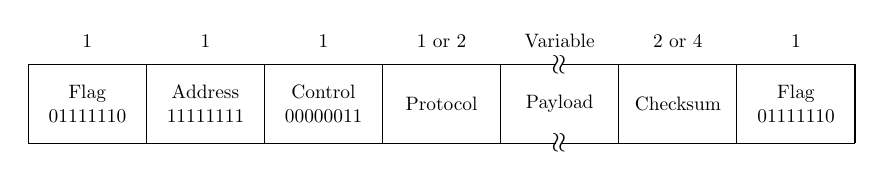
\begin{tikzpicture}
        %%%%%%%% Blocchi %%%%%%%%%
        \draw (0,0) -- ++(6.7,0) ++ (.08,0) -- (10.5,0);
        \draw (0,1) -- ++(6.7,0) ++ (.08,0) -- (10.5,1);
        \node[rotate=90] at (6.75,0) {$\approx$};
        \node[rotate=90] at (6.75,1) {$\approx$};

        \foreach \x in {0,1.5,...,10.5}
            \draw (\x,0) -- ++(0,1);

        %%%%%%%%% Testo %%%%%%%%%%
        \node[align=center,text width=1.4cm,scale=0.7] at (0.75,0.5) {Flag 01111110};
        \node[align=center,text width=1.4cm,scale=0.7] at (2.25,0.5) {Address 11111111};
        \node[align=center,text width=1.4cm,scale=0.7] at (3.75,0.5) {Control 00000011};
        \node[align=center,text width=1.4cm,scale=0.7] at (5.25,0.5) {Protocol};
        \node[align=center,text width=1.4cm,scale=0.7] at (6.75,0.5) {Payload};
        \node[align=center,text width=1.56cm,scale=0.7] at (8.25,0.5) {Checksum};
        \node[align=center,text width=1.4cm,scale=0.7] at (9.75,0.5) {Flag 01111110};

        \foreach \x in {0.75,2.25,3.75,9.75}
            \node[scale=0.7] at (\x,1.3) {1};

        \node[scale=0.7] at (5.25,1.3) {1 or 2};
        \node[scale=0.7] at (6.75,1.3) {Variable};
        \node[scale=0.7] at (8.25,1.3) {2 or 4};

    \end{tikzpicture}
\end{center}